\documentclass[12pt]{article}
\usepackage[utf8]{inputenc}
\usepackage[margin=1in]{geometry}
\usepackage[spanish]{babel}\decimalpoint
\usepackage{setspace}\onehalfspacing
\usepackage{parskip} %Espacio entre parrafos.
\usepackage{graphicx} %Para usar \includegraphics[]{}
\usepackage{amssymb} %Para usar el simbolo del conj. de los Reales.%
\usepackage{amsmath} % Para usar columnas vectoriales.
\usepackage{multirow}
\usepackage{hyperref} %Siempre debe ser el ultimo paquete.


\setcounter{tocdepth}{2} %Que no incluya subsubsections en el índice.

%================================

\title{Clase 19: Teorema Fundamental del Cálculo (Parte 1).}
\author{MIT 18.01: Single Variable Calculus.}
\date{}

\begin{document}

\maketitle

\begin{abstract}
\noindent Como se señaló en la clase anterior, las integrales definida y indefinida se relacionan a pesar de sus diferencias. Esto se da por medio del \textbf{Teorema Fundamental del Cálculo}. En esta clase abordaremos una parte de éste, así como en las propiedades de las integrales definidas que podemos obtener con él. Su relevancia es tal que, desde ahora, lo usaremos para resolver integrales definidas en vez de la suma de Riemann.
\end{abstract}


\section{Teorema Fundamental del Cálculo (TFC 1).}

Las integrales definida e indefinida se vinculan o unen en el siguiente teorema.

\textbf{Teorema.} Si $f(x)$ es una función continua y se cumple que $F'(x) = f(x)$, entonces:
\[
  \int_{a}^{b} f(x)dx = F(b) - F(a)
\]
Veamos que la igualdad de arriba se cumple solo si $F(x)$ es la antiderivada de $f(x)$, pero luego toma como entrada los límites de la integral definida, por tanto pasa a ser un número y no una familia de funciones. Lo anterior corresponde al \textbf{Teorema Fundamental del Cálculo}.

Este teorema se denota de forma más resumida como:
\[
  \int_{a}^{b} f(x) dx = \left.F(x)\right|_{x = a}^{x = b} = \left.F(x)\right|_{a}^{b} = F(b) - F(a)
\]
Cuando trabajamos con más de una variable, lo mejor es poner explícitamente en los límites la variable con la que estamos trabajando, pero en caso contrario, no es necesario.

Resolver una integral definida a partir del TFC 1 es mucho más fácil, porque solo tenemos que aplicar las propiedades de las antiderivadas que hemos estudiado. Veámoslo con uno de los ejemplos de la clase anterior.

\textbf{Ejemplo 1.} \quad Calcule $\int_{0}^{b} x^{2} dx$ usando el TFC 1.

\textbf{Solución.} \quad Para resolver esta integral, solo tenemos que aplicar la propiedad de las potencias de las integrales indefinidas.
\[
  \int_{0}^{b} x^{2} dx = \left.\left(\frac{x^{2 + 1}}{2 + 1}\right)\right|_{0}^{b}
                        = \frac{b^{3}}{3} - \frac{0^{3}}{3}
                        = \frac{b^{3}}{3}
\]
Como vemos, el esfuerzo aplicado fue excesivamente menor en relación a la clase anterior.

\textbf{Ejemplo 2.} \quad Calcule el área sombreada de la función $\sin(x)$.

\begin{figure}[hbt!]
\centering
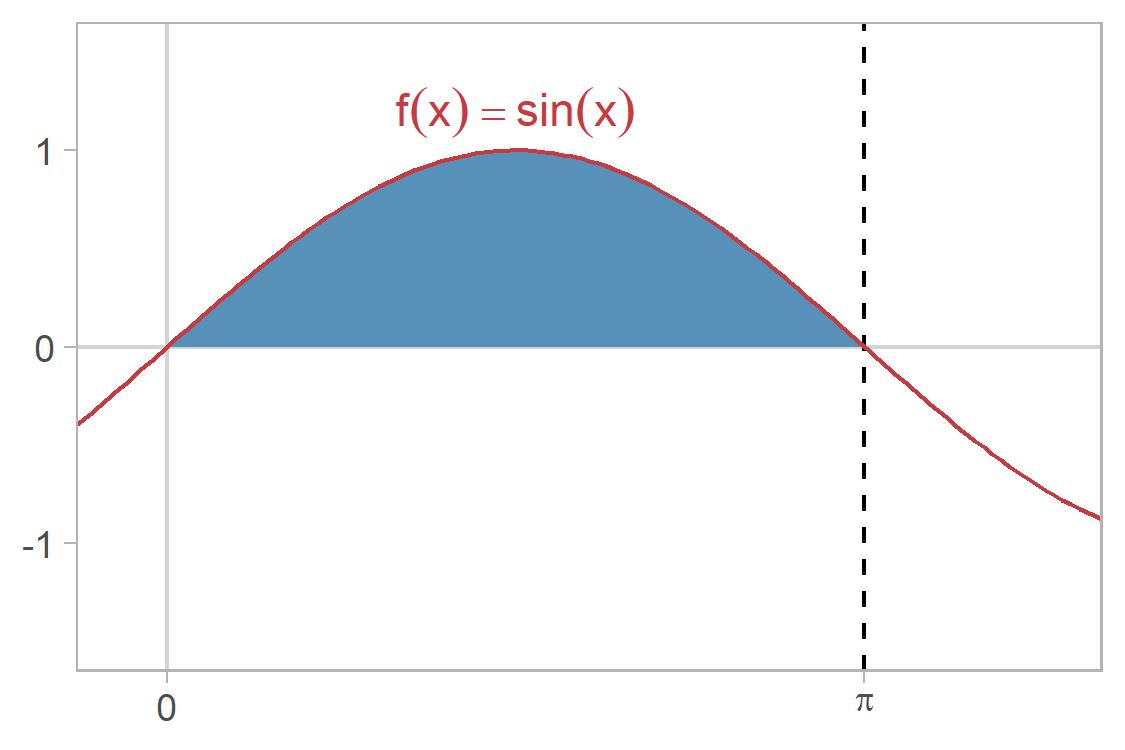
\includegraphics[scale=0.7]{img/def-int-sin.jpg}
\end{figure}

\textbf{Solución.} \quad En este caso nos piden calcular la integral del $\sin(x)$ entre $[0, \ \pi]$. Aquello es mucho más fácil de resolver con el TFC 1.
\[
  \int_{0}^{\pi} \sin(x) = \left.-\cos(x)\right|_{0}^{\pi}
                         = -\cos(\pi) - (-\cos(0))
                         = -(-1) - (-1)
                         = 2
\]

\subsection{La integral definida como la distancia recorrida entre dos puntos.}

A partir del TFC 1, podemos interpretar a la integral definida como la distancia recorrida desde un punto a otro.

Supongamos que vamos a un evento, desde un punto $a$ (nuestra casa) hasta $b$, donde la distancia en función del tiempo es dada por $x(t)$ y su rapidez por $x'(t) = v(t)$.

Durante el viaje vamos tan obsesionados con el tiempo que iremos revisando un reloj a cada segundo. En ese sentido, la distancia en un segundo cualquiera podemos medirla como:
\[
  v(t) \Delta t
\]
Si medimos la distancia a cada segundo desde $a$ hasta $b$, entonces la distancia recorrida al $i$-ésimo segundo del viaje será la suma de las distancias individuales.
\[
  \sum_{i = 1}^{n} v(t_{i}) \Delta t
\]
Independiente de la distancia del viaje, es evidente que nos tomará una cantidad enorme de segundos, por tanto podemos asumir que la suma de arriba se aproximará a la integral definida la que, por el \textbf{TFC 1}, será \textbf{exactamente igual a la distancia recorrida desde $a$ hasta $b$}.
\[
  \sum_{i = 1}^{n} v(t_{i}) \Delta t \approx \int_{a}^{b} v(t) dt = x(b) - x(a)
\]

\subsection{Interpretación geométrica completa de la Integral Definida.}

Geométricamente, a la integral definida la hemos entendido como el área bajo la curva de una función y sobre el eje horizontal. El problema con esta interpretación, es que se queda incompleta cuando el área está sobre la curva y bajo el eje.

Por ejemplo, calculemos la integral definida del $\sin(x)$ entre $[0, \ 2\pi]$.
\[
  \int_{0}^{2\pi} \sin(x)dx = -\cos(x)|_{0}^{2\pi} = -\cos(2\pi) - (-\cos(0)) = -1 + 1 = 0 
\]
A partir de la gráfica del $\sin(x)$ y de su integral que vemos a continuación, podríamos decir que el cálculo de arriba es errado porque sí hay un área. En realidad, es igual a cero porque una parte de dicha superficie es \textbf{negativa}\footnote{En realidad un área de signo negativo es algo que no tiene sentido, pero ya veremos cuándo eso ocurre.} y, por ese motivo, resulta en aquel valor.

\begin{figure}[hbt!]
\centering
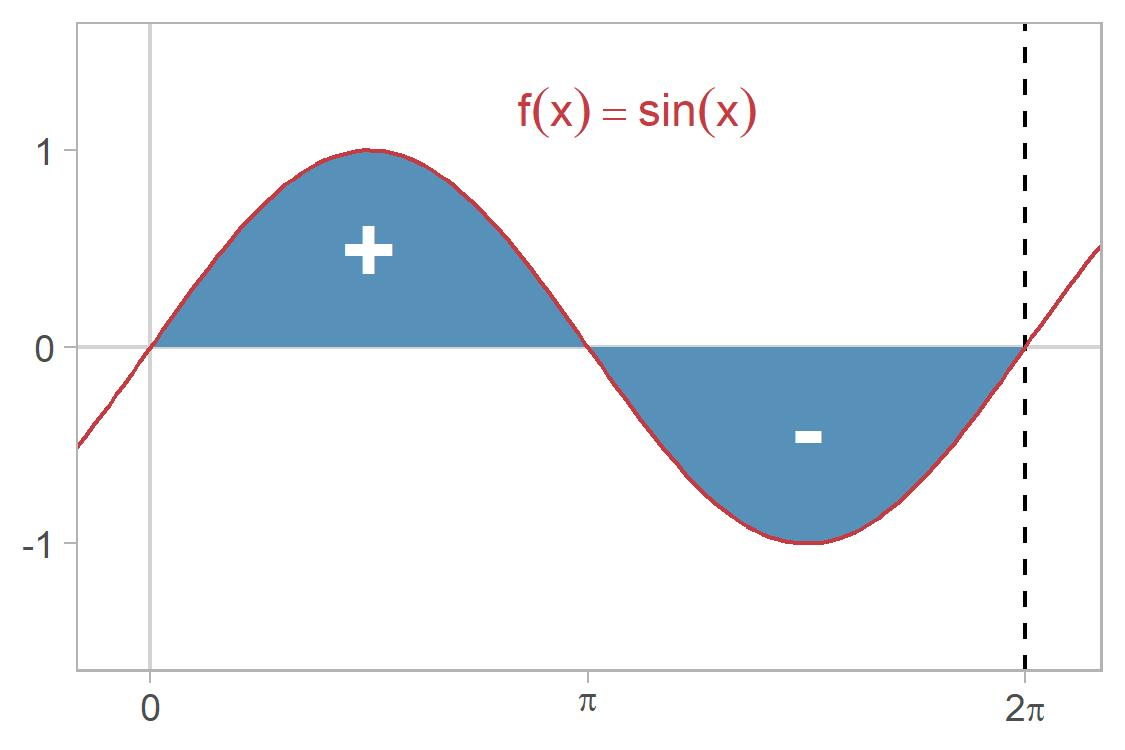
\includegraphics[scale=0.7]{img/def-int-sin-2.jpg}
\end{figure}

Entonces, la interpretación geométrica completa de la integral definida es \textbf{el área positiva sobre el eje horizontal y bajo la curva, menos el área bajo el mismo eje y sobre la curva}.

Esto también podemos verlo a partir del ejemplo de la sección anterior.

Consideremos ahora la dirección en el viaje, lo que significa que la tasa de cambio de la distancia con respecto al tiempo corresponde a la velocidad\footnote{Para este ejemplo, asumamos que es de una dimensión o un componente.} o $x'(t) = \vec{v}(t)$. Supongamos que justo a mitad del trayecto nos avisan que el evento se suspendió por motivos personales, así que tuvimos que devolvernos a nuestra casa, cumpliéndose que $x(a) = x(b)$. Por lo tanto:
\[
  \int_{a}^{b} \vec{v}(t) dt = x(b) - x(a) = 0
\]
Esto no significa que nos quedamos estáticos, más bien quiere decir que no hubo cambio en la posición porque en el trayecto tuvimos que movernos en sentido contrario (i.e, en ese momento $\vec{v}(t) < 0$), volviendo al punto inicial. Es por ello que la suma acumulada de las distancias terminó anulándose.

La integral de arriba corresponde al \textbf{desplazamiento} o la \textbf{distancia neta recorrida}, que es el \textbf{cambio en la posición} del vehículo y que, por tanto, considera a la velocidad $\vec{v}(t)$. Por otra parte, si queremos conocer \textbf{la longitud del camino recorrido} a pesar del cambio de dirección, calculamos la \textbf{distancia recorrida total} por medio del valor absoluto de la velocidad, $|\vec{v}(t)|$, que no es sino la \textbf{rapidez}, que fue lo que vimos en la sección anterior.

\section{Propiedades de las Integrales Definidas.}

\subsection{Propiedades Básicas.}

Las siguientes dos propiedades de las integrales son las más sencillas y no requieren explicación:
\begin{align*}
&1. \, \int_{a}^{b} (f(x) \pm g(x))dx = \int_{a}^{b} f(x)dx \pm \int_{a}^{b} g(x)dx \\
&2. \, \int_{a}^{b} c \cdot f(x)dx = c \cdot \int_{a}^{b} f(x)dx 
\end{align*}
Otra propiedad, es que si los límites $a = b$, entonces la integral es cero:
\[
3. \, \int_{a}^{a} f(x)dx = 0
\]
Esto se explica tanto geométricamente, porque el área se hace infinitamente delgado, como por el TFC1, ya que $\int_{a}^{a} f(x)dx = F(a) - F(a) = 0$.

La siguiente propiedad es una interesante.
\[
4. \, \int_{a}^{b} f(x)dx = - \int_{b}^{a} f(x)dx
\]
A nivel geométrico, la integral de la derecha de la igualdad sin considerar el signo $(-)$, no existe porque el área de cualquier figura siempre debe ser positivo. No obstante, esta propiedad es \textbf{consistente con el TFC 1}.
\begin{align*}
  \int_{a}^{b} f(x)dx &= - \int_{b}^{a} f(x)dx \\
  F(b) - F(a) &= - (F(a) - F(b)) \\
  F(b) - F(a) &= F(b) - F(a)
\end{align*}
Una quinta propiedad de las integrales, es la que sigue:
\[
5. \ \int_{a}^{b} f(x)dx + \int_{b}^{c} f(x)dx = \int_{a}^{c} f(x)dx
\]
Podemos notar en la igualdad de arriba que, en el lado izquierdo, estamos asumiendo que $a < b < c$, pero \textbf{a partir de la propiedad $4.$ esto no es necesario} para que se cumpla. Por ejemplo, también es válido escribir la propiedad de la siguiente manera:
\[
  \int_{b}^{a} f(x)dx + \int_{b}^{c} f(x)dx = \int_{a}^{c} f(x)dx
\]
La sexta propiedad que veremos a continuación, se conoce como \textbf{Estimación}:
\[
6. \, \int_{a}^{b} f(x)dx \leq \int_{a}^{b} g(x)dx \iff f(x) \leq g(x)
\]
En este caso necesariamente debe cumplirse que $a < b$, de lo contrario debemos cambiar el orden de la desigualdad.

\textbf{Ejemplo 3.} \quad Demuestre que $e^{x} \geq 1$ para todo $x \geq 0$.

\textbf{Solución.} \quad Este ejemplo es un caso de la propiedad de \textbf{estimación}. Apliquemos la integral definida en la desigualdad, asumiendo que $a = 0$ y que $b \geq 0$.

\begin{align*}
  \int_{0}^{b} e^{x}dx &\geq \int_{0}^{b} 1dx \\
  e^{b} - 1 &\geq b \\
  e^{b} &\geq b + 1
\end{align*}
Algo a tener en cuenta es que corresponde a la propiedad de estimación solo si $b \geq 0$, en caso contrario, si $b < 0$, se cumple la desigualdad de arriba, pero no la propiedad.

\subsection{Método de Sustitución en Integrales Definidas.}

Cuando el integrando es una función compuesta, podemos aplicar el método de sustitución, que es similar al usado en las integrales indefinidas.

Sean $u = g(x)$, $u_{1} = g(x_{1})$, $u_{2} = g(x_{2})$ y $du = g'(x)dx$. Entonces:
\[
  \int_{u_{1}}^{u_{2}} f(u)du = \int_{g(x_{1})}^{g(x_{2})} f(g(x)) \cdot g'(x)dx
\]
Veamos ahora lo relevante que es tener en cuenta a la variable en los límites de la integral, porque deben cambiar si aplicamos este método si no queremos alterarla.

\textbf{Ejemplo 4.} \quad Calcule $\int_{1}^{2} (x^{3} + 2)^{5} x^{2} dx$.

\textbf{Solución.} \quad Podemos aplicar el método de sustitución, estableciendo que $u = x^{3} + 2$, lo que significa que $du = 3x^{2}dx$, $u_{1} = 1^{3} + 2 = 3$ y $u_{2} = 2^{3} + 2 = 10$, obteniendo que:
\[
  \int_{1}^{2} (x^{3} + 2)^{5} x^{2} dx = \int_{3}^{10} \frac{1}{3} u^{5}du
                                        = \frac{1}{3} \cdot \left.\frac{u^{6}}{6}\right|_{3}^{10}
                                        = \left.\frac{u^{6}}{18}\right|_{3}^{10}
                                        = \frac{10^{6}}{18} - \frac{3^{6}}{18}
\]
Algo a tener en cuenta, es que el método de sustitución en integrales definidas solo funcionará si $g'(x)$ \textbf{nunca cambia su signo}. No es que de ocurrir aquello el método estará errado, sino que induce muy fácilmente a equivocarnos. Veámoslo en el siguiente ejemplo.

\textbf{Ejemplo 5.} \quad Calcule $\int_{-1}^{1} x^{2}dx$ usando el método de sustitución, asumiendo que $u = x^{2}$.

\textbf{Solución.} \quad Comencemos aplicando el método de sustitución a partir de la información que nos dan, donde $du = 2xdx$, $u_{1} = 1$ y $u_{2} = 1$.
\[
  \int_{-1}^{1} x^{2}dx = \int_{1}^{1} \frac{1}{2x}udu
\]
La igualdad de arriba es errada, porque el lado derecho es igual a cero, pero el izquierdo no lo es y podemos demostrarlo a partir del TFC 1. Esto ocurre porque $2x$, que es la derivada de $x^{2}$, cambia de signo cuando $x > 0$ y $x < 0$.

Esto podemos identificarlo aún más si, en el lado derecho, reemplazamos $x = \sqrt{u}$.
\[
  \int_{-1}^{1} x^{2}dx = \int_{1}^{1} \frac{1}{2\sqrt{u}}udu
\]
el cual en realidad es $x = \pm \sqrt{u}$.

Entonces lo coherente sería tener dos fórmulas para el lado derecho, una para $+ \sqrt{u}$ y otra para $- \sqrt{u}$. Aun así es mucho más probable, en este caso, equivocarnos al aplicar el método de sustitución, por lo tanto lo mejor es evitarlo. Sobretodo acá, donde podríamos haberlo resuelto más rápido con el TFC 1.

\end{document}
